% !TEX root = ../main.tex
\section{Limitations and Conclusion}
\label{sec:limitations}
Our closed-loop evidence is in simulation on one robot and four objects, with replayed depth for the offline study; SafeLIBERO and the real robot (Secs.~\ref{sec:safelibero}--\ref{sec:real}) widen this but do not remove it. The precise surface does not yet convert into higher success than the coarse exemption on the hurdle set, and the cause is not isolated: our arm changes extent and robot mask together, and neither the simulator's own target surface nor the volume mask alone recovers the failures. Whether the identity alert changes any closed-loop outcome is unmeasured; in the held-out runs it withheld \pend{43} chunks whose outcome we have not attributed. The prototype runs at about \pend{0.35}\,Hz chunk rate (\pend{2.9}\,s per request); the dominant cost, the per-request surface graph, is amenable to caching and GPU construction, and the duplicated backbone pass can be shared. We reconstruct observed surfaces only: the scene field treats unobserved space as free, so occluded geometry, missing depth, and sub-voxel contacts remain unresolved, and robot-depth matching needs accurate meshes and kinematics. Query coverage is bounded by the sphere model: with a post directly beside the target, both the frozen policy and \sys\ touched it because the real hand surface lay 13--39\,mm outside the modeled spheres (Fig.~\ref{fig:failure}). The reassociation can preserve a wrong first reference, which is what the two worsened held-out episodes show, and the supervised phase model uses effectively floor-referenced height. A hold is an intervention, not a safety certificate.

\begin{figure}[t]
\centering
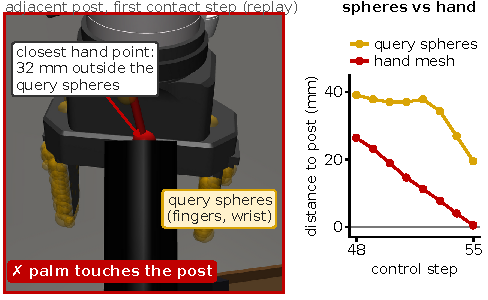
\includegraphics[width=\columnwidth]{../figures/cvpr_v1/fig07_failure.pdf}
\caption{\textbf{Failure case: coverage, not grounding.} With a post directly beside the target, the palm rests on the post at the first contact (red point) while every constraint sphere stays clear of it; the hand point closest to the post lies \pend{32}\,mm outside the sphere union. The frozen policy alone makes the same contact.}
\label{fig:failure}
\end{figure}

A frozen VLA already says which object it is about to touch and what stage of the task it is in; it does not know where that object's surface ends or which of its own links may enter it. \sys\ keeps these questions apart and answers each with the evidence that can: attention seeds, depth continuity bounds, centered features re-identify, physical feedback authorizes, and link-specific fields carry the answers into constrained execution, without an external segmenter or any change to the policy. We see this separation of evidence as what lets geometric safety layers and learned policies share a scene rather than one overruling the other.
